\section{Indledning}

Tekst.\\

Tekst.\\

Tekst.\\




\subsection{Problemformulering}

Tekst
\begin{itemize}
	\item Tekst
	\item Tekst
	\item Tekst
\end{itemize}

\subsection{Kravspecifikation}

TekstTekstTekstTekstTekst\\
TekstTekst\\
TekstTekstTekst \footnote{Test footnote}\\
Tekst

\begin{itemize}
	\item Tekst
	\item Tekst
	\item Tekst

\end{itemize}

%Signatur til matematik
\[(5)+5=10\]


$\displaystyle \sum$


$\displaystyle \int x^5+b_1$


$\frac{n!}{k!(n-k)!} = \binom{n}{k}$

\subsection{Projektafgrænsning}

Tekst

\begin{itemize}
	\item Tekst
	\item Tekst
	\item Tekst
\end{itemize}

Tekst


\subsection{Tidsplan}

\begin{figure}[h]
	\centering
		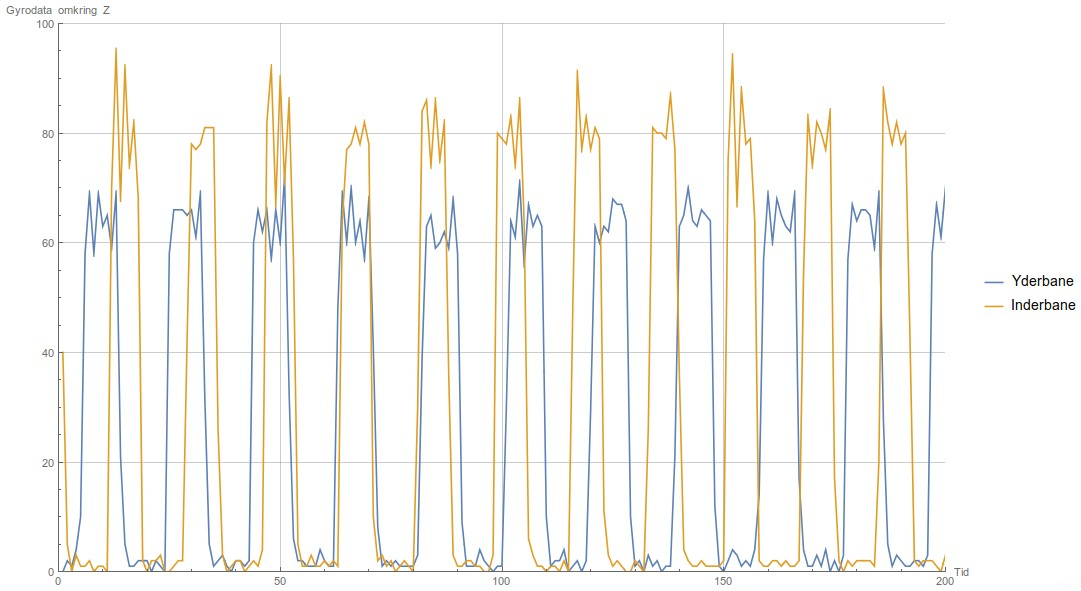
\includegraphics[scale=0.75]{Billeder/Gyro.jpg}
	\caption{Her kan vi se vores tidsplan}
	\label{fig:tidsplan}
\end{figure}